\documentclass[conference,9pt]{IEEEtran}
\usepackage{xcolor}
\usepackage{cite}
\usepackage{epsfig}
\usepackage{amssymb}
\usepackage{amsmath}
\usepackage{graphicx}
\graphicspath{ {./} }

\begin{document}
\title{Practical 2}

\author{
\IEEEauthorblockN{Albert Acebron}
\IEEEauthorblockA{NIU: 1458626}
}


% make the title area
\maketitle
\begin{abstract}
In this practical we'll analyze several of the techniques used to estimate parameters of a signal that has been corrupted by noise and use them to provide an estimate of the values that have the highest likelihood of generating a matching signal.
\end{abstract}



%----------------------------------------------------------------
% SECTION #1 
\section{Introduction}

We know that white noise follows a gaussian distribution, so if we have a signal that has been corrupted by it, it shouldn't be hard to conclude that a given realization of it taken at a specific time will have the same probability distribution, with the caveat that it's center will be situated at the actual value of the signal. 

That is, given a realization of a signal at a given time $s(t)$ and it's corrupted variant $s(t)+w_i$, the distribution of it will match that of a gaussian centered around $s(t)$.

Now, if our signal is non-constant\footnote{And is not cyclic with a period that matches the sampling interval, which would make it appear as if it was constant once sampled} this distribution will change depending on the time $t$, since $s(t)$ will be different and that will alter the center of the gaussian. So if we wanted to get the probability distribution of a sample that could have been taken at a time $t\in [0, N-1]$ we'd need to get the probability distributions of the first $N$ samples and multiply them together.

Putting it in numbers, if we had a signal such as:
$$x(n) = Acos(2 \pi f_d n + \phi ) + w_i(n)$$

We could take the probability distribution of a gaussian function:

$$f(x)=\frac{1}{\sigma\sqrt{2\pi}}e^{-\frac{(x-\mu_x)^2}{2\sigma^2}}$$

And swap $\mu_x$ with our signals value at a point in time to get the pdf\footnote{Probability density function} of a realization of our signal at that time:

$$f(x)=\frac{1}{\sigma\sqrt{2\pi}}e^{-\frac{(x-Acos(2 \pi f_d n + \phi ))^2}{2\sigma^2}}$$

And if we wanted to get the pdf of a sample that could have been taken at multiple times we'd just multiply several of these functions together as mentioned before, resulting in:

$$f(x)=\frac{1}{(\sigma\sqrt{2\pi})^N}e^{-\frac{\sum_{n=0}^{N-1}(x(n)-Acos(2 \pi f_d n + \phi ))^2}{2\sigma^2}}$$

However, in this practical we will use a single realization at a specific time for most of our exercises, so we will only use the former pdf.

\section{Simple estimation}
Given multiple realizations taken from a signal such as the one described before at $n=0$, where the parameters $A$ and $\sigma$ are known but we want to estimate $\phi$, a simple method of going about it would be to graph the probability distributions that we would get with different values of $\phi$ and then compare those with the distribution of values seen in our realizations.

Here's the graph\footnote{See appendix for code, note that from here on onwards all the graphs will have their accompanying code available on the Appendix} of the pdfs associated with $\frac{\pi}{4}$, $\frac{\pi}{2}$ and $\frac{3\pi}{2}$:

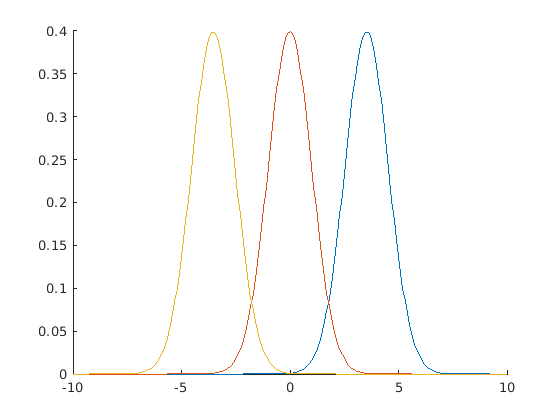
\includegraphics[scale=0.6]{3}

And here's it superposed with a histogram of the realizations at $n=0$:


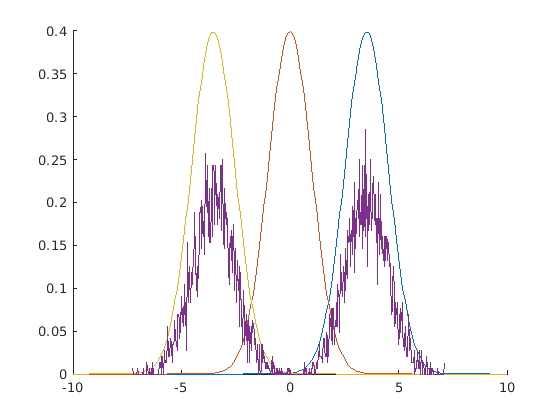
\includegraphics[scale=0.6]{4}

We can appreciate that the pdf that fits better our experimental data is the one associated with $\phi=\frac{3\pi}{4}$, which will be our estimation.

We must also note that the samples we used for our histogram were from different points in the space domain but from the same one on the time domain, as if we had taken samples at different times these would have differing pdfs\footnote{See the explanation on the Introduction section}, so we'd get a histogram that would be the result of mixing multiple pdfs.

Note that if the process that we are evaluating was ergodic we'd actually be able to pick values from the time and space domain indistictly, but it's not so we must stick with the space domain to maintain $N=1$ and the same pdf in all of our samples.

\section{Continuous estimation}

While in the previous case our estimate proved to be correct, in cases where we don't have any clue about the possible values of $\phi$ this method wouldn't be useful (or would only get us very crude estimates with larga amounts of work) as we won't have at hand a set of possible values to compare against, instead $\phi$ could take any value.

Luckily in these cases we can rely on a different method, which works in the following way:

If we go back to the formula of a single pdf provided on the Introduction and analyze it again, we can interpret it as a function that, given a possible value of our signal, tells us how likely it is that a sample would fall on any value.

Until right now we've used this function with fixed values for our signal values, which provided us with the pdf for samples of that signal (at that time), but we could reverse the roles and instead use make the sample fixed and evaluate the function for different possible values of the function. This would give us, for every value evaluated, the probability that our sample to be the value it is if our signal had a specific value at that point in time.

Analytically, this means that, given a sample $y$ we will use the following function to calculate the likelihood that a given $\phi$ was used:
$$f(\phi)=\frac{1}{\sigma\sqrt{2\pi}}e^{-\frac{(y-Acos(2 \pi f_d n + \phi ))^2}{2\sigma^2}}$$

That might seem a bit confusing but the net effect is that, for values of the signal where the result of the function is low it is very unlikely that our random sample would have occurred, whereas for high values a sample like that is likely to appear.

To illustrate the point better, let's take the first realization at time $n=0$ of our signal and graph our likelihood function applied to it:
  
  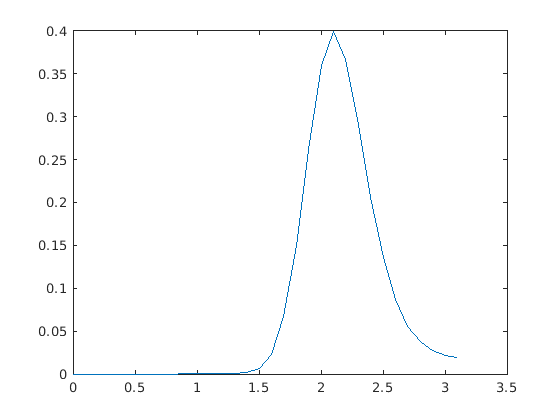
\includegraphics[scale=0.6]{nou6}

We can appreciate that the values with highest likelihood fall around 2, but to find the specific value that would be provided by an ML estimation we can apply it's definition and select the value that represents the maximum, which in the case of this specific sample is $2.2$.

Now, if we repeat the same process with different realizations we will get the following estimations:

\begin{center}
    \begin{tabular}{ c c }
    RxSignal(1,2) & 3  \\ 
    RxSignal(1,3) & 2.3  \\  
    RxSignal(1,4) & 2.7  \\  
    RxSignal(1,5) & 2   
    \end{tabular}
\end{center}

As we can see, these estimations have some variability due to the fact that only a single sample is used for each one of them, so any deviation caused by noise will directly affect our result (eg: atypical realization leads to skewed estimate). One way to solve that would be to aggregate the result of a lot of different estimations that use different realizations, as that allows the law of big numbers to kick in and makes the noise less relevant since we clearly see what's more statistically likely.

This is what we'll be doing in the following sections.

\section{Improved ML estimation}
Previously we've been calculating ML estimations using a single realization and calculating all values to pick their maximum later, which is extremely inefficient. In this section we will improve our estimates by first using many more samples ($N>1$ which means we will be using the pdf derived from multpiplying together the pdfs of multiple gaussians) and by optimizing the calculations through thanks to the following analytical reasoning:

Let's remember that the an ML estimation is just finding a maximum of the function
$$f(\phi|x)=\frac{1}{(\sigma\sqrt{2\pi})^N}e^{-\frac{\sum_{n=0}^{N-1}(x(n)-\mu_{x(n)})^2}{2\sigma^2}}$$

One way to do that would be by using the classic method of differentiating the function against $\phi$, equating the result to zero and solving the resulting equation.

But this is quite complex to do, so instead we will make use of the fact that $ln$ is an strictly increasing function to optimize $-ln(f\phi|x)$ instead, as, due to that property mentioned before, the latter function will only have a minimum if and only if the former has a maximum at the same point\footnote{This can be proved by taking into account the minus sign, which inverts minimums and maximums and the fact that $ln(x)$ will be maximum when $x$ is maximum, as if there existed a number $y$ such that $ln(y)>ln(x)$ then $y>x$ due to the strictly increasing nature of $ln$, and thus $x$ wouldn't be maximum, reaching a reducting to absurdity}. Meaning that, if we manage to find a value for which $-ln(f(\phi|x))$ is minimum that'll be the maximum we were searching for.

With this new function we can use several of the properties of logarithms and differentiation to cancel a bunch of constant terms and get a much nicer equation to work with, which when solved for 0 as partial derivative of $\phi$ results in the following equation\footnote{When the signal being estimated is given by the equation that was provided in Introduction} for the estimated $\phi$:

$$\phi=-arctan(\frac{\sum_{n=0}^{N-1}x(n)cos(2\pi f_n n)}{\sum_{n=0}^{N-1}x(n)cos(2\pi f_n n)})$$

Before continuing, we'll synthetically generate a signal, to use as the basis of all our following tests, that matches the one we described in our Introduction, has $\phi=1$ and the power of it's complex noise is unitary. 

And, to get unitary noise, we'll have to force the variance of the noise to be 1.

Now, the definition of variance is $var=E[(X-\mu)^2]$, where $\mu$ is the mean of $X$, and because $X$ is gaussian noise, it's mean will be 0, so $var=E[X^2]$.

Forcing $var=1$ we get to the point where we need to force the expected value of $X^2$ to be one, and one way to do it is by forcing all $X$ to just be $1$. Given that this is the easiest solution and it can be applied with a single scaling factor we'll apply it dividing all the values by their absolute value in order to force their absolute value to be 1.

Wrapping it all together, we'll use the following code to generate our test signal:
\begin{verbatim}
    fd=0.25;
    A=5;
    N=10000;
    n=(1:N)';
    noise=randn(N, 1) + randn(N, 1)*i;
    noise=noise./abs(noise);
    x=A*cos(2*pi*fd.*n + 1) + noise;
\end{verbatim}

After generating it, let's start by running a few estimations on it\footnote{Code available in Appendix} with amount of samples ($N$) at different magnitudes:

\begin{center}
    \begin{tabular}{ c c }
    N & estimate  \\ 
    100 & 1.0170 - 0.0457i  \\  
    1000 & 1.0027 - 0.0096i  \\  
    10000 & 1.0016 + 0.0001i
    \end{tabular}
\end{center}

We can appreciate that, as we theorized in the previous section where ML estimation was introduced, using a higher number of samples has reduced significantly the errors that noise causes on the estimations as even with only $N=100$ the predictions are pretty accurate (significantly more than our previous predictions that used a single sample). What's more, as $N$ grows, the accuracy of our predictions improves, which logically makes sense since more samples are getting used and this makes any noise less statistically rellevant.

Now that we've taken a glimpse at the results of our estimator we will proceed to do a short analysis on the properties of it, starting by making 1000 estimations with $N=1000$ and plotting the resulting estimates:

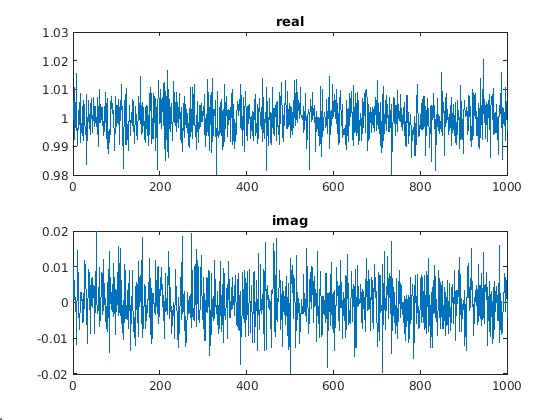
\includegraphics[scale=0.6]{b5}

As we've seen previously, the results provided are pretty close to the real value of $\theta = 1$, but in this plot we can observe something new: There's quite some variance in the results, as all estimations on this plot are for the same value but they are spread on a range. We believe this is caused by the estimation error incurred in different realizations due to the noise, but we'll do one more experiment before issuing any conclusion.

To confirm our suspicions, we'll recreate our previous experiment but with multiple values of $N$ at several magnitudes, more concretely at $N=100$ (blue), $N=1000$ (red) and $N=10000$ (yellow):

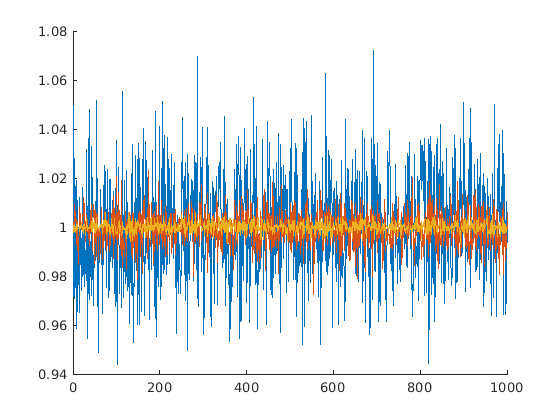
\includegraphics[scale=0.6]{b6}

Looking at the graph, it's easy to see that as $N$ grows the variance in our results that we noticed before, and therefore the error present them, gets smaller, and observaction that is confirmed by the following aggregate metrics:

\begin{center}
  \begin{tabular}{ c c c }
   N & Bias & Variance \\ 
   100 & 7.0954e-04 - 1.5122e-04i & 5.4412e-04 \\  
   1000 & -4.7884e-04 + 1.4569e-04i & 5.8087e-05 \\  
   10000 & -9.5291e-05 - 1.3311e-05i & 5.4140e-06  
  \end{tabular}
\end{center}

These metrics also support the thesis that, as $N$ grows, both bias and variance, along with the errors incurred, decrease, meaning that, on aggregate, the higher $N$ is, the closer our estimations will be to the real value.

Again, this is just another data point behind the theory we've formulated several times: Due to the nature of statistical processes (and especially gaussian noise, which cancels itself out as $N$ approaches infinity because of the fact that it's mean is 0) a higher amount of samples and realizations included into our calculations will result in lower errors and lower variance on our estimations, as random processes tend to even themselves out when a sufficiently large amount of samples is aggregated.

\section{Error metrics}
To wrap it up, we'll calculate the MSE of our estimations, a metric that takes into account their variance and bias to produce a single number that is used as a quantitative metric on the quality of the estimations, the lower the better. Then, we'll compare this with the Cramér-Rao Lower Bound, which is the optimal accuracy that can be generated by unbiased estimator, in other words, the theoretical optimal bound.

Graphed onto the same canvas for direct comparison, here our estimator's MSE (red) and CRLB (blue) by $N$:

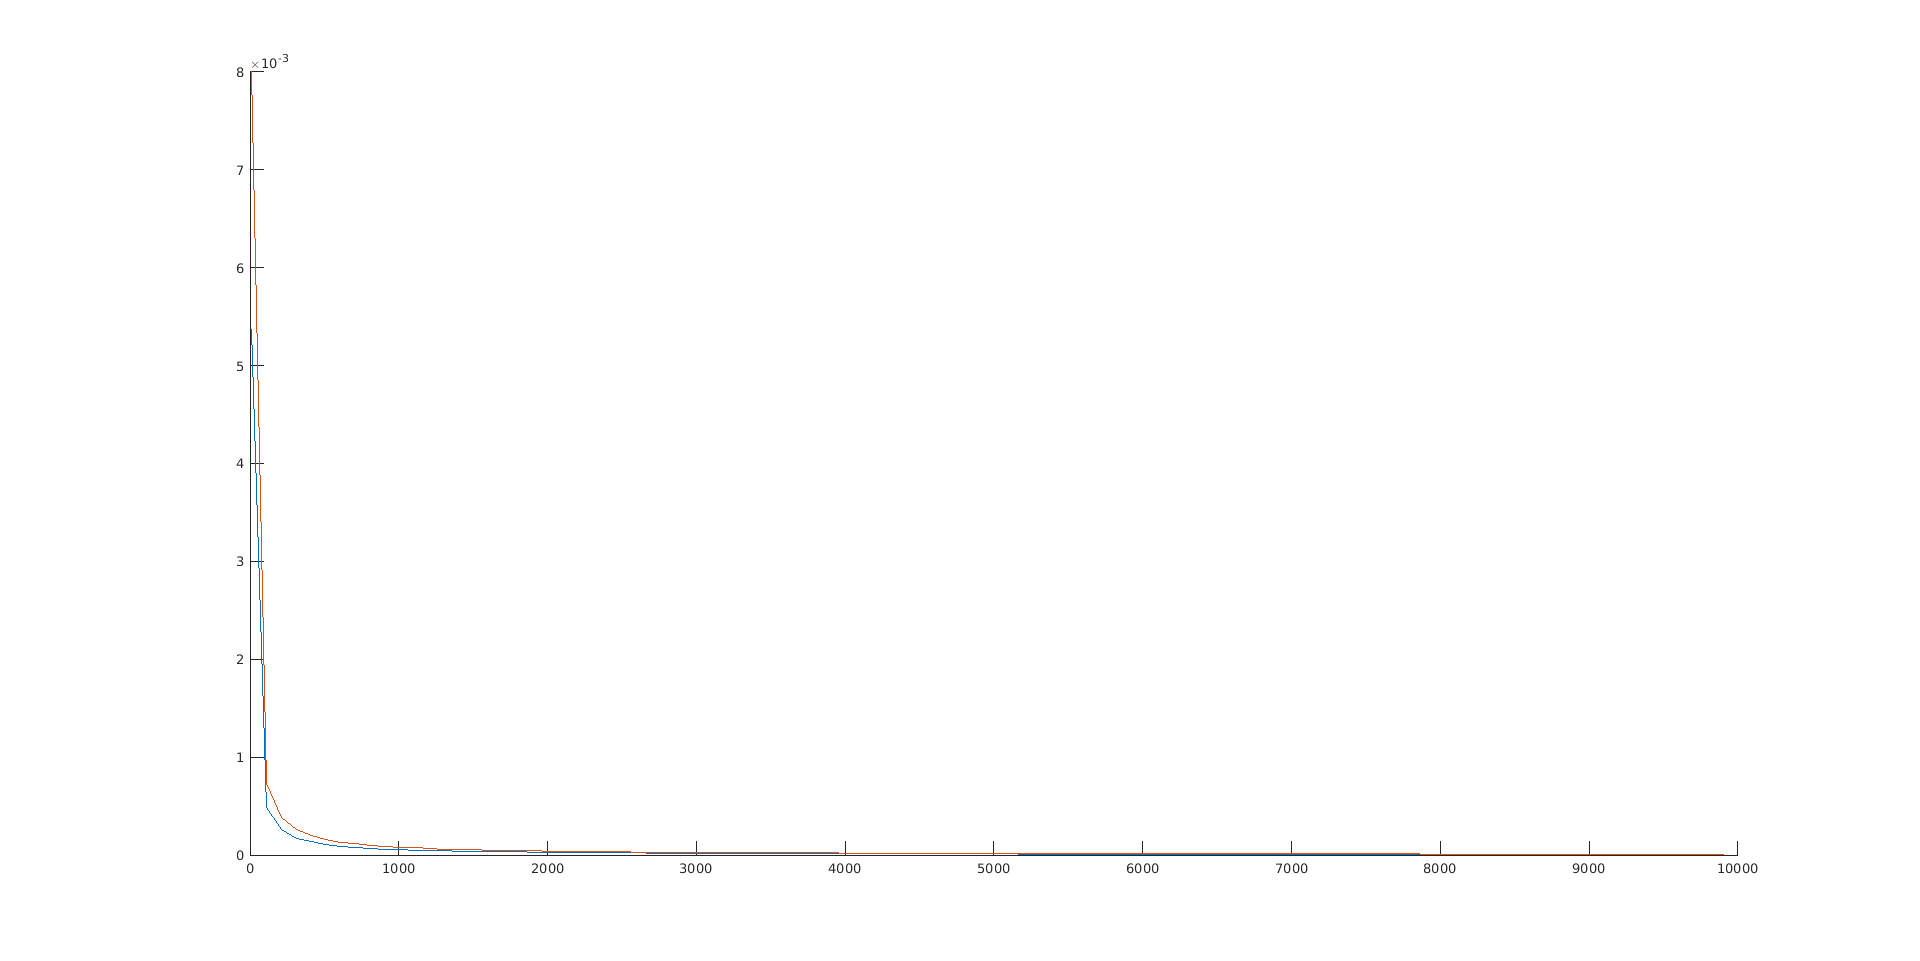
\includegraphics[scale=0.18]{b7}

On this plot we can observe that our MSE follows closely the CRLB, meaning that our predictions are quite good as they are close to the theoretical optimum, thus our ML estimator is efficient.

Furthermore, we can appreciate how both MSE and CRLB increase sharply when getting close to really low values of N such as $10$ whereas they both decrease for larger values. This is in line with the thesis that we've been repeating through this whole paper, that a higher $N$ implies more data points that make it much harder for an anomaly to cause an estimation error. On the other side, if the number of data points is really low the probability of noise misleading the estimator is much higher since it's much harder for the noise to even itself out.

On top of that, we can also conclude that the ML estimator is consistent, as it's bias stays generally quite low.

Finally, with this last piece of evidence that directly links a quality metric with the value of $N$ in a directly proportional way, we conclude that we've collected enough evidence to make a strong case for the theory that we've proposed on this paper.

\section{Conclusion}
In this paper we've analyzed and applied successfully several techniques for estimating parameters of a function, we've put forward the thesis that a higher amount of samples leads to less error-prone predictions and we've finally proved it with empirical evidence.

\section{Appendix}
\subsection{Graph of different pdfs for different values of $\phi$}
\begin{verbatim}
    x = -10:0.1:10;
    sigma = 1;
    hold on;
    mu = 5*cos(pi/4);
    y = (1/(sigma*sqrt(2*pi)))
      .*exp(-((x-mu).^2)/(2*sigma^2));
    plot(x,y)
    mu = 5*cos(pi/2);
    y = (1/(sigma*sqrt(2*pi)))
      .*exp(-((x-mu).^2)/(2*sigma^2));
    plot(x,y)
    mu = 5*cos(3*pi/4);
    y = (1/(sigma*sqrt(2*pi)))
      .*exp(-((x-mu).^2)/(2*sigma^2));
    plot(x,y)
  \end{verbatim}

\subsection{Graph of the histogram}
  \begin{verbatim}
    r=RxSignal(1,:);
    d=500;
    [h, x]=hist(r,d);
    lr=length(r);
    lh=x(end)-x(1)
    plot(x,h.*(d/(lr*lh)));
  \end{verbatim}

 \subsection{Graph of likelihood function}
 \begin{verbatim}
    x=0:0.1:pi;
    y = (1/(sigma*sqrt(2*pi))).*exp(
      -((RxSignal(1,1)-5*cos(x)).^2)/(2*sigma^2));
    plot(x,y);
  \end{verbatim}

\subsection{ML estimation}
Run the code that calculates the likelihood function (previous section) and afterwards:
  \begin{verbatim}
    find(y==max(y))/10
   \end{verbatim}

\subsection{Computing ML estimates}
We'll initially define an estimation script/function:
\begin{verbatim}
    function [theta] = estimate(n, x, fd)
      upper=sum(x.*sin(2*pi*fd*n));
      lower=sum(x.*cos(2*pi*fd*n));
      theta=-atan(upper./lower);
    end
\end{verbatim}

And apply it:

\begin{verbatim}
  theta1 = estimate(n(1:100), x(1:100), fd)
  theta2 = estimate(n(1:1000), x(1:1000), fd)
  theta3 = estimate(n(1:10000), x(1:10000), fd)
\end{verbatim}

\subsection{Plot 1000 estimates}

\begin{verbatim}
    N=1000;
    n=(1:N)';
    thetas = zeros(1000, 1);
    for c=1:1000
      noise=randn(N, 1) + randn(N, 1)*i;
      noise=noise./abs(noise);
      x=A*cos(2*pi*fd.*n + 1) + noise;
      thetas(c) = estimate(n, x, fd);
    end
    subplot(2,1,1)
    plot(real(thetas))
    title('real')
    subplot(2,1,2)
    plot(imag(thetas))
    title('imag')
  \end{verbatim}

\subsection{Plot multiple estimates for different values of N}

\begin{verbatim}
    function [] = plot6(N)
      n=(1:N)';
      K=1000;
      thetas = zeros(K, 1);
      for c=1:K
        noise=randn(N, 1) + rand(N, 1)*i;
        noise=noise./abs(noise);
        x=A*cos(2*pi*fd.*n + 1) + noise;
        thetas(c) = estimate(n, x, fd);
      end
      plot(abs(thetas))
      N
      bias=mean(thetas')-1
      variance=var(thetas')
    
    % Execute
    hold on
    b6(100)
    b6(1000)
    b6(10000)
    \end{verbatim}

\subsection{Compute MSE and CRLB}
Given that $\sigma_w = 1$ due to the fact that we imposed that on question 1, we'll get that $CRLB=\frac{2}{NA^2}$:

\begin{verbatim}
  nn=10:100:10000;    
  MSEs = zeros(length(nn), 1);
  CRLBs = zeros(length(nn), 1);
  for N=nn
    n=(1:N)';
    K=1000;
    thetas = zeros(K, 1);
    for c=1:K
      noise=randn(N, 1) + rand(N, 1)*i;
      noise=noise./abs(noise);
      x=A*cos(2*pi*fd.*n + 1) + noise;
      thetas(c) = estimate(n, x, fd);
    end
    bias=mean(thetas')-1;
    variance=var(thetas');
  
    c=ceil(N/100);
    CRLBs(c)=2/(N*A^2);
    MSEs(c)=real(bias)^2+variance;
  end
  hold on
  plot(nn, MSEs)
  plot(nn, CRLBs)
\end{verbatim}


\end{document}


